\section{Appendix}

\subsection{Code Listings}

\subsubsection{Alpha Testing Script}
\begin{lstlisting}[language=C++, caption=Alpha Testing Script]
class AlphaTest {
public:
    // Test modes
    enum TestMode {
        MOTOR_TEST,
        SENSOR_TEST,
        ENCODER_TEST,
        IMU_TEST,
        TAG_TEST
    };

    void runTest(TestMode mode) {
        switch(mode) {
            case MOTOR_TEST:
                testMotorSequence();
                break;
            case SENSOR_TEST:
                testSensors();
                break;
            case ENCODER_TEST:
                testEncoders();
                break;
            case IMU_TEST:
                testIMU();
                break;
            case TAG_TEST:
                testAprilTag();
                break;
        }
    }

private:
    void testMotorSequence() {
        // Test each motor individually
        Serial.println("Testing Front Motor");
        testSingleMotor(RPWM_RIGHT, LPWM_RIGHT);
        Serial.println("Testing Left Motor");
        testSingleMotor(RPWM_LEFT, LPWM_LEFT);
        Serial.println("Testing Back Motor");
        testSingleMotor(RPWM_BACK, LPWM_BACK);
        // Test combined movements
        // ... additional code ...
    }
    
    // ... additional test methods ...
};
\end{lstlisting}

\subsubsection{Final Implementation Excerpt}
\begin{lstlisting}[language=C++, caption=Robot Controller Class]
class RobotController {
public:
    enum OperationMode {
        MANUAL,
        AUTONOMOUS,
        TAG_FOLLOWING,
        CHARGING
    };
    
    RobotController() : currentMode(MANUAL) {
        setupHardware();
        calibrateSensors();
    }
    
    void run() {
        while(true) {
            updateSensors();
            processCommands();
            updateState();
            controlLoop();
            reportStatus();
            delay(50); // 20Hz update rate
        }
    }

private:
    OperationMode currentMode;
    bool emergencyStopped = false;
    unsigned long lastUpdate = 0;
    
    void setupHardware() {
        // Initialize all pins
        setupMotors();
        setupSensors();
        setupCommunication();
        Serial.println("Hardware initialization complete");
    }
    
    // ... additional methods ...
};

// Main program
RobotController robot;

void setup() {
    Serial.begin(115200);
    Wire.begin();
    robot = RobotController();
}

void loop() {
    robot.run();
}
\end{lstlisting}

\subsection{Technical Drawings}

\begin{figure}[H]
    \centering
    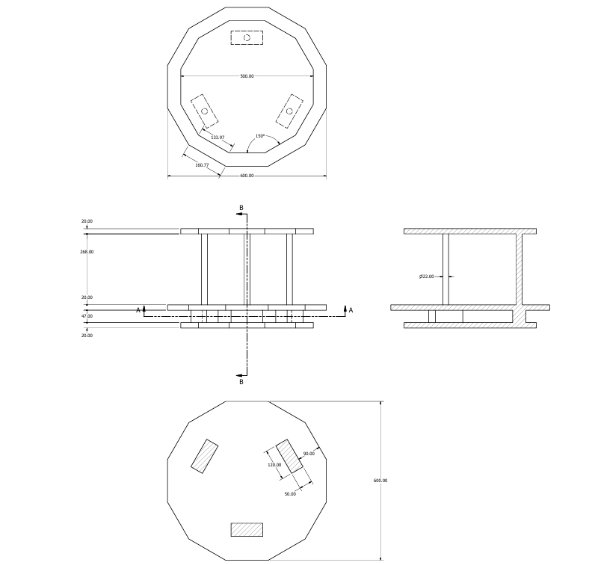
\includegraphics[width=0.7\linewidth]{../ReportMovementModule/images/Aspose.Words.728084da-df58-4b9d-a372-f65cffbdb23d.008.jpeg}
    \caption{Structure Technical Drawings}
\end{figure}

\subsection{Component List}

\begin{itemize}
    \item 3 × JGB37-520 12V DC Motors with encoders
    \item 3 × 58mm Omnidirectional wheels
    \item 3 × DRV8871 Motor drivers
    \item 1 × ATmega328P Microcontroller board
    \item 6 × HC-SR04 Ultrasonic distance sensors
    \item 1 × 11.1V 2200mAh LiPo battery
    \item 1 × LM2596 DC-DC Step-down power regulator
    \item 1 × Camera module
    \item Various wooden panels, supports, and fasteners
    \item LED strips for illumination
    \item Cotton padding and white fabric for aesthetic covering
    \item Transparent tube for ticket dispensing mechanism
    \item Decorative elements for the robot character
\end{itemize}

\subsection{Testing Procedures}

During development, we performed a series of standardized tests to validate the movement module's functionality:

\begin{enumerate}
    \item \textbf{Motor calibration}: Testing each motor individually with varying PWM values to ensure consistent response and power consumption.
    \item \textbf{Sensor validation}: Measuring detection ranges and accuracy of ultrasonic sensors at different distances and angles.
    \item \textbf{Movement patterns}: Verifying basic movements (forward, backward, lateral, and rotational) followed by combined motions.
    \item \textbf{Obstacle detection}: Running the robot in controlled environments with strategically placed obstacles to test avoidance behaviors.
    \item \textbf{Battery endurance}: Measuring operational time under various movement patterns to estimate effective patrol duration.
    \item \textbf{AprilTag detection}: Testing the reliability and range of visual marker recognition in different lighting conditions.
\end{enumerate}

These tests were performed iteratively throughout development, with results informing subsequent design refinements and optimizations.
